\documentclass[a4paper]{article}

\usepackage[english]{babel}
\usepackage{amsfonts, amssymb, mathtools, amsthm, amsmath}
\usepackage{graphicx, pgfplots}
\usepackage{bm} 
\usepackage{url}
\usepackage[dvipsnames]{xcolor}
\usepackage{lastpage}
\usepackage{chngcntr}
  \counterwithin{figure}{section}
  \renewcommand{\thefigure}{\thesection.\arabic{figure}}

%loaded last
\usepackage[hidelinks]{hyperref}
\usepackage[nameinlink]{cleveref} 

\usepackage{siunitx}
  \sisetup{exponent-product = \cdot,
    output-decimal-marker = {,}}

%Giles Castelles incfig
\usepackage{import}
\usepackage{xifthen}
\usepackage{pdfpages}
\usepackage{transparent}

\newcommand{\incfig}[2][1]{%
  \def\svgwidth{#1\columnwidth}
  \import{./figures/}{#2.pdf_tex}
}

\setlength{\parindent}{0in}
\setlength{\parskip}{12pt}
\setlength{\oddsidemargin}{0in}
\setlength{\textwidth}{6.5in}
\setlength{\textheight}{8.8in}
\setlength{\topmargin}{0in}
\setlength{\headheight}{18pt}

\usepackage{fancyhdr}
\pagestyle{fancy}

\fancyhead{}
\fancyfoot{}
\fancyfoot[R]{\thepage}
\fancyhead[C]{\leftmark}

\pgfplotsset{compat=newest}

\pgfplotsset{every axis/.append style={
  axis x line=middle,    % put the x axis in the middle
  axis y line=middle,    % put the y axis in the middle
  axis line style={<->,color=black}, % arrows on the axis
}}

\usepackage{thmtools}
\usepackage{tcolorbox}
  \tcbuselibrary{skins, breakable}
  \tcbset{
    space to upper=1em,
    space to lower=1em,
  }

\theoremstyle{definition}

\newtcolorbox[auto counter]{definition}[1][]{%
  breakable,
  colframe=ForestGreen,  %frame color
  colback=ForestGreen!5, %background color
  colbacktitle=ForestGreen!25, %background color for title
  coltitle=ForestGreen!70!black,  %title color
  fonttitle=\bfseries\sffamily, %title font
  left=1em,              %space on left side in box,
  enhanced,              %more options
  frame hidden,          %hide frame
  borderline west={2pt}{0pt}{ForestGreen},  %display left line
  title=Definition \thetcbcounter: #1,
}

\newtcolorbox{greenline}{%
  breakable,
  colframe=ForestGreen,  %frame color
  colback=white,          %remove background color
  left=1em,              %space on left side in box
  enhanced,              %more options
  frame hidden,          %hide frame
  borderline west={2pt}{0pt}{ForestGreen},  %display left line
}

\newtcolorbox[auto counter, number within=section]{dis}[1][]{%
  breakable,
  colframe=NavyBlue,  %frame color
  colback=NavyBlue!5, %background color
  colbacktitle=NavyBlue!25,    %background color for title
  coltitle=NavyBlue!70!black,  %title color
  fonttitle=\bfseries\sffamily, %title font
  left=1em,            %space on left side in box,
  enhanced,            %more options
  frame hidden,        %hide frame
  borderline west={2pt}{0pt}{NavyBlue},  %display left line
  title=Discussion \thetcbcounter: #1
}

\newtcolorbox{blueline}{%
  breakable,
  colframe=NavyBlue,     %frame color
  colback=white,         %remove background
  left=1em,              %space on left side in box,
  enhanced,              %more options
  frame hidden,          %hide frame
  borderline west={2pt}{0pt}{NavyBlue},  %display left line
}

\newtcolorbox{exa}[1][]{%
  breakable,
  colframe=RawSienna,  %frame color
  colback=RawSienna!5, %background color
  colbacktitle=RawSienna!25,    %background color for title
  coltitle=RawSienna!70!black,  %title color
  fonttitle=\bfseries\sffamily, %title font
  left=1em,              %space on left side in box,
  enhanced,              %more options
  frame hidden,          %hide frame
  borderline west={2pt}{0pt}{RawSienna},  %display left line
  title=Example: #1,
}

\newtcolorbox[auto counter, number within=section]{sæt}[1][]{%
  breakable,
  colframe=RawSienna,  %frame color
  colback=RawSienna!5, %background color
  colbacktitle=RawSienna!25,    %background color for title
  coltitle=RawSienna!70!black,  %title color
  fonttitle=\bfseries\sffamily, %title font
  left=1em,              %space on left side in box,
  enhanced,              %more options
  frame hidden,          %hide frame
  borderline west={2pt}{0pt}{RawSienna},  %display left line
  title=Sætning \thetcbcounter: #1,
  before lower={\textbf{Bevis:}\par\vspace{0.5em}},
  colbacklower=RawSienna!25,
}

\newtcolorbox{redline}{%
  breakable,
  colframe=RawSienna,  %frame color
  colback=white,       %Remove background color
  left=1em,            %space on left side in box,
  enhanced,            %more options
  frame hidden,        %hide frame
  borderline west={2pt}{0pt}{RawSienna},  %display left line
}

\newtcolorbox{des}[1][]{%
  breakable,
  colframe=NavyBlue,  %frame color
  colback=NavyBlue!5, %background color
  colbacktitle=NavyBlue!25,    %background color for title
  coltitle=NavyBlue!70!black,  %title color
  fonttitle=\bfseries\sffamily, %title font
  left=1em,              %space on left side in box,
  enhanced,              %more options
  frame hidden,          %hide frame
  borderline west={2pt}{0pt}{NavyBlue},  %display left line
  title=Description of #1,
}

\makeatother
\def\@lecture{}%
\newcommand{\lecture}[3]{
  \ifthenelse{\isempty{#3}}{%
    \def\@lecture{Lecture #1}%
  }{%
    \def\@lecture{Lecture #1: #3}%
  }%
  \subsection*{\makebox[\textwidth][l]{\@lecture \hfill \normalfont\small\textsf{#2}}}
}

\makeatletter

\newcommand{\exercise}[1]{%
 \def\@exercise{#1}%
 \subsection*{Exercise #1}
}

\makeatother

%Format lim the same way in intext and in display
\let\svlim\lim\def\lim{\svlim\limits}

% horizontal rule
\newcommand\hr{
\noindent\rule[0.5ex]{\linewidth}{0.5pt}
}

\author{Noah Rahbek Bigum Hansen}



\title{Prøveeksamen – Termodynamik}
\date{26. Maj 2025}

\begin{document}

\maketitle

\opgave{1.}
Luft ved \qty{25}{\celsius} ekspanderes i en adiabatisk proces fra et volumen på \qty{1}{L} til \qty{2}{L}. Bestem tryk, densitet og specifik enthalpi i sluttilstanden.
\bigbreak
Vi antager at trykket i starttilstanden er atmosfæretryk, $p_1 = \qty{101,325}{kPa}$. Såfremt det antages at processen er isentropisk kan de velkendte sammenhænge fra isentropiske processer bruges:
\begin{align*}
  \frac{P_2}{P_1} &= \left( \frac{V_1}{V_2} \right)^{\gamma} \\
  \frac{T_2}{T_1} &= \left( \frac{V_1}{V_2} \right)^{\gamma - 1}
.\end{align*}
For at finde densiteten antages at luften er en idealgas og derfor kan idealgasloven benyttes som:
\[ 
\rho_2 = \frac{P_2}{R T_2}
.\]
Entalpien for luften kan slutteligt findes som:
\[ 
h_2 = c_p T_2
.\]
Dette er regnet I EES som:
\begin{verbatim}
  gamma = 1,4
  R = 0,287 [kJ/kg K]
  cp = gamma*R/(gamma - 1)
  T1 = 298 [K]
  P1 = 101,325 [kPa]
  V1 = 0,001 [m3]
  V2 = 0,002 [m3]
   
  T2 = T1*(V1/V2)^(gamma - 1)
  P2 = P1*(V1/V2)^gamma
  rho2 = P2/(R*T2)
  h2 = cp*T2
\end{verbatim}
EES giver her et resultat på $p_2 = \qty{38,39}{kPa}$, $\rho_2 = \qty{0,5924}{\frac{kg}{m^3}} $ og $h_2 = \qty{227,2}{\frac{kJ}{kg}}$. 

\opgave{2.}
En turbine har følgende egenskaber: en isentropisk virkningsgrad på 83\%, et indgangstryk på \qty{30}{bar}, et udgangstryk på \qty{80}{bar}, og en udgangstemperatur på \qty{327}{\celsius}. Arbejdsmediet er damp og massestrømmen gennem turbinen er \qty{20}{kg/s}. Bestem dampens indgangstemperatur og arbejdet turbinen kan udføre.
\bigbreak
Idet vi har to tilstandstørrelser til sluttilstanden kan vi regne de resterende vha. stofdatakald i EES således fås:
\begin{align*}
  h_2 &= \qty{3113}{\frac{kJ}{kg}}  \\
  s_2 &= \qty{7,38}{\frac{kJ}{kg\cdot K}} 
.\end{align*}
Desuden kan den isentropiske virkningsgrad regnes som:
\[ 
\eta_{\mathrm{is}} = \frac{h_1 - h_2}{h_1 - h_{2s}} = \num{0,83} 
.\]
Heri kan $h_{2s}$ regnes vha. et stofdatakald i EES som:
\begin{verbatim}  
  h_s[2] = enthalpy(Water;P=P[2];s=s[1])
\end{verbatim}
Dermed er den eneste ubekendte i formlen for $\eta_{\mathrm{is}}$ altså $h_1$. Denne kan iterativt findes i EES ved at gætte på en starttemperatur. Dette giver en temperatur $T_1 = \qty{588}{\celsius}$ for at den isentropiske virknignsgrad passer med den angivne værdi. Dermed er to tilstandsstørrelser også kendt for begyndelsestilstanden, hvorved de resterende kan findes vha. stofdatakald i EES til hhv.
\begin{align*}
  h_1 &= \qty{3523}{\frac{kJ}{kg}}  \\
  s_1 &= \qty{7,205}{\frac{kJ}{kg\cdot K}} \\
  h_{2,s} &= \qty{3078}{\frac{kJ}{kg}} 
.\end{align*}

Dermed kan det specifikke arbejde udført af turbinen findes som:
\[ 
w = h_1 - h_2 = \qty{3523}{\frac{kJ}{kg}} - \qty{3154}{\frac{kJ}{kg}} = \qty{369}{\frac{kJ}{kg}} 
.\]
Og dermed kan den samlede effekt findes som:
\[ 
\dot{W} = \qty{20}{\frac{kg}{s}} \cdot \qty{369}{\frac{kJ}{kg}} = \qty{7,38}{MW} 
.\]


\opgave{3.}
Damp ved \qty{150}{\celsius} og atmosfærisk tryk anvendes til at fjerne is fra nogle køleribber. Umiddelbart før afrimningen har isen en gennemsnitstemperatur på \qty{-3}{\celsius} og en masse på \qty{2}{kg}. Antag at dampen kun udveksler varme med isen og at dampen forlader systemet med en kvalitet på 80\%. Bestem den samlede mængde af damp som er nødvendigt for at smelte alt isen.
\bigbreak
Der kan opstilles en energibalance idet energien der skal bruges af isen må være summen af den energi det kræves at opvarme isen fra \qty{-3}{\celsius}  til \qty{0}{\celsius} og den energi det kræver at smelte isen. Dette må altså være:
\[ 
  Q_{\mathrm{ice}} = m_{\mathrm{ice}}\cdot \left( h_{\mathrm{ice}} + h_{f, \mathrm{ice}}\right)
.\]
Idet vi både har trykket og temperaturen på isen i starten og ved smeltepunktet kan begge entalpi-værdier findes vha. stofdatakald i EES.

Energien frigivet pr. kilogram damp er lig entalpiforskellen på dampen før og efter det har passeret igennem systemet. Begge disse kan findes med stofdatakald i EES. Dernæst kan massen af damp påkrævet regnes som:
\[ 
m_s = \frac{Q_{\mathrm{ice}}}{\Delta h}
.\]
Dette er gjort i EES, hvorved massen af damp påkrævet er fundet til $m_s = \qty{1,228}{kg}$. 


\opgave{4.}
En varmemaskine arbejder mellem temperaturniveauerne \qty{250}{\celsius} og \qty{10}{\celsius}. Den får tilført \qty{10}{MW} varme ved den høje temperatur og afgiver \qty{3}{MW} varme ved den lave temperatur. Resten bliver omdannet til arbejde. Argumenter for om det kan lade sig gøre ift. termodynamikkens første og anden lov.
\bigbreak
Termodynamikkens 1. lov er om energibevarelse. I dette tilfælde tilføres der mere energi end der afgives idet $E_{\text{tilført}} = \qty{10}{MW} > E_{\text{afgivet}} = \qty{3}{MW}$. Dermed er der intet problematisk ift. den 1. lov.

Termodynamikkens 2. lov foreskriver bl.a. at varmemaskiner ikke kan have en virkningsgrad bedre end Carnots virkningsgraden for en tilsvarende proces. I dette tilfælde er den egentlige virkningsgrad for varmemaskinen:
\[ 
\eta_{\text{egentlig}} = \frac{\dot{W}}{\dot{Q}_H} = \frac{\qty{7}{MW}}{\qty{10}{MW}} = 70\%
.\]
Carnot virkningsgraden for en tilsvarende proces er:
\[ 
\eta_{\mathrm{carnot}} = 1 - \frac{T_L}{T_H} = 1 - \frac{\qty{283}{K}}{\qty{523}{K}} = \num{45,9}\%
.\]
Dermed er virkningsgraden for maskinen bedre end den teoretisk optimale og dermed bryder maskinen termodynamikkens 2. lov. 


\opgave{5.}
Tegn et procesdiagram for en gasmotor som anvender en Brayton kredsproces. Motoren skal kunne anvende spildvarmen fra udstødningsgassen til fjernvarme og anvende to kompressorer med mellemkøling. Angiv mindst 4 relevante tilstandsnumre og et groft bud på tryk og temperatur i de nummererede tilstande.
\bigbreak
\begin{figure}[ht]
  \centering
  \incfig[0.8]{p1_2}
  \caption{Procesdiagram}
  \label{fig:p1-2}
\end{figure}
På \textbf{\autoref{fig:p1-2}} ses et bud på procesdiagrammet for processen. Her optages atmosfærisk luft i tilstand 1, hvorfor $T_1 = \qty{20}{\celsius}$ og $p_1 = \qty{1}{bara}$. I tilstand 2 er dette blevet komprimeret i det første komprimeringstrin. Her er et bud på temperatur og tryk hhv. $T_2 = \qty{140}{\celsius}$ $p_2 = \qty{3,16}{bara} $. I tilstand 3 er gassen blevet ført igennem turbinen og dermed må det have et tryk tæt på $p_3 = \qty{1}{bar} $ her er temperaturen nok fortsat høj, omend ikke så høj som i brændselskammeret. Et bud på en temperatur kunne være $T_3 = \qty{600}{\celsius}$. I tilstand 4 er dette blevet røggaskølet og her er temperaturen nok ikke meget over $T_4 = \qty{100}{\celsius}$ ved et tryk på $p_4 = \qty{1}{bara}$.

\opgave{6.}
Indtegn følgende proces på et passende $T$-$s$-diagram og $P$-$v$-diagram: $\mathrm{CO}_2$ ved et tryk på \qty{1}{bar} og en temperatur på \qty{100}{\celsius} afkøles til \qty{40}{\celsius} ved en isobar process. Herefter komprimeres gassen adiabatisk og isentropisk til et tryk på \qty{50}{bar}. Til slut afkøles gassen ved konstant volumen til \qty{15}{\celsius}.
\bigbreak
Følgende EES kode er blevet fremstillet til at beregne alle tilstandsstørrelser:
\begin{verbatim}
  P[1] = 1              [bar]
  T[1] = 100           [C]
  s[1] = Entropy(CarbonDioxide;P=P[1];T=T[1])
  v[1] = volume(CarbonDioxide;P=P[1];T=T[1]) 
 
  P[2] = P[1]
  T[2] = 40             [C]
  s[2] = Entropy(CarbonDioxide;P=P[2];T=T[2])
  v[2] = volume(CarbonDioxide;P=P[2];T=T[2])
 
  P[3] = 50             [bar]
  s[3] = s[2]
  T[3] = temperature(CarbonDioxide;P=P[3];s=s[3])
  v[3] = volume(CarbonDioxide;P=P[3];s=s[3])
 
  v[4] = v[3]
  T[4] = 15             [C]
  P[4] = pressure(CarbonDioxide;T=T[4];v=v[4])
  s[4] = entropy(CarbonDioxide;T=T[4];v=v[4])
\end{verbatim}
Med afsæt i resultatet af dette kan de to nedenstående diagrammer fremstilles. 
\begin{figure} [ht]
  \centering
  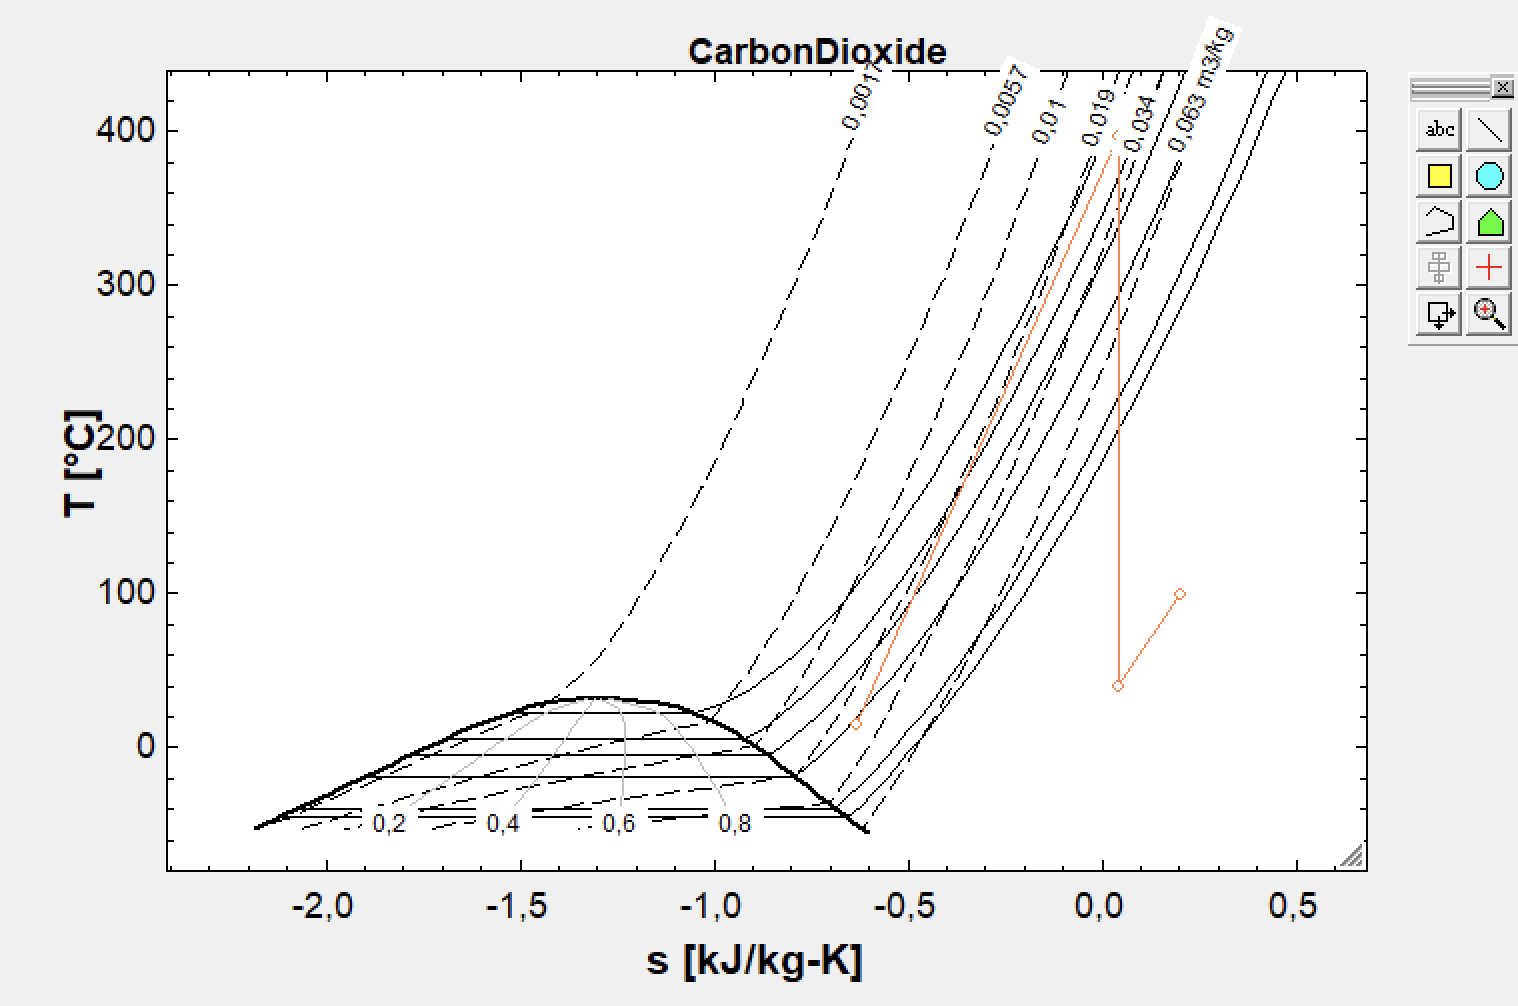
\includegraphics[width=0.5\linewidth]{./figures/p1_3.png}
  \caption{$Ts$-diagram}
  \label{fig:p1_3}
\end{figure}

\begin{figure} [ht]
  \centering
  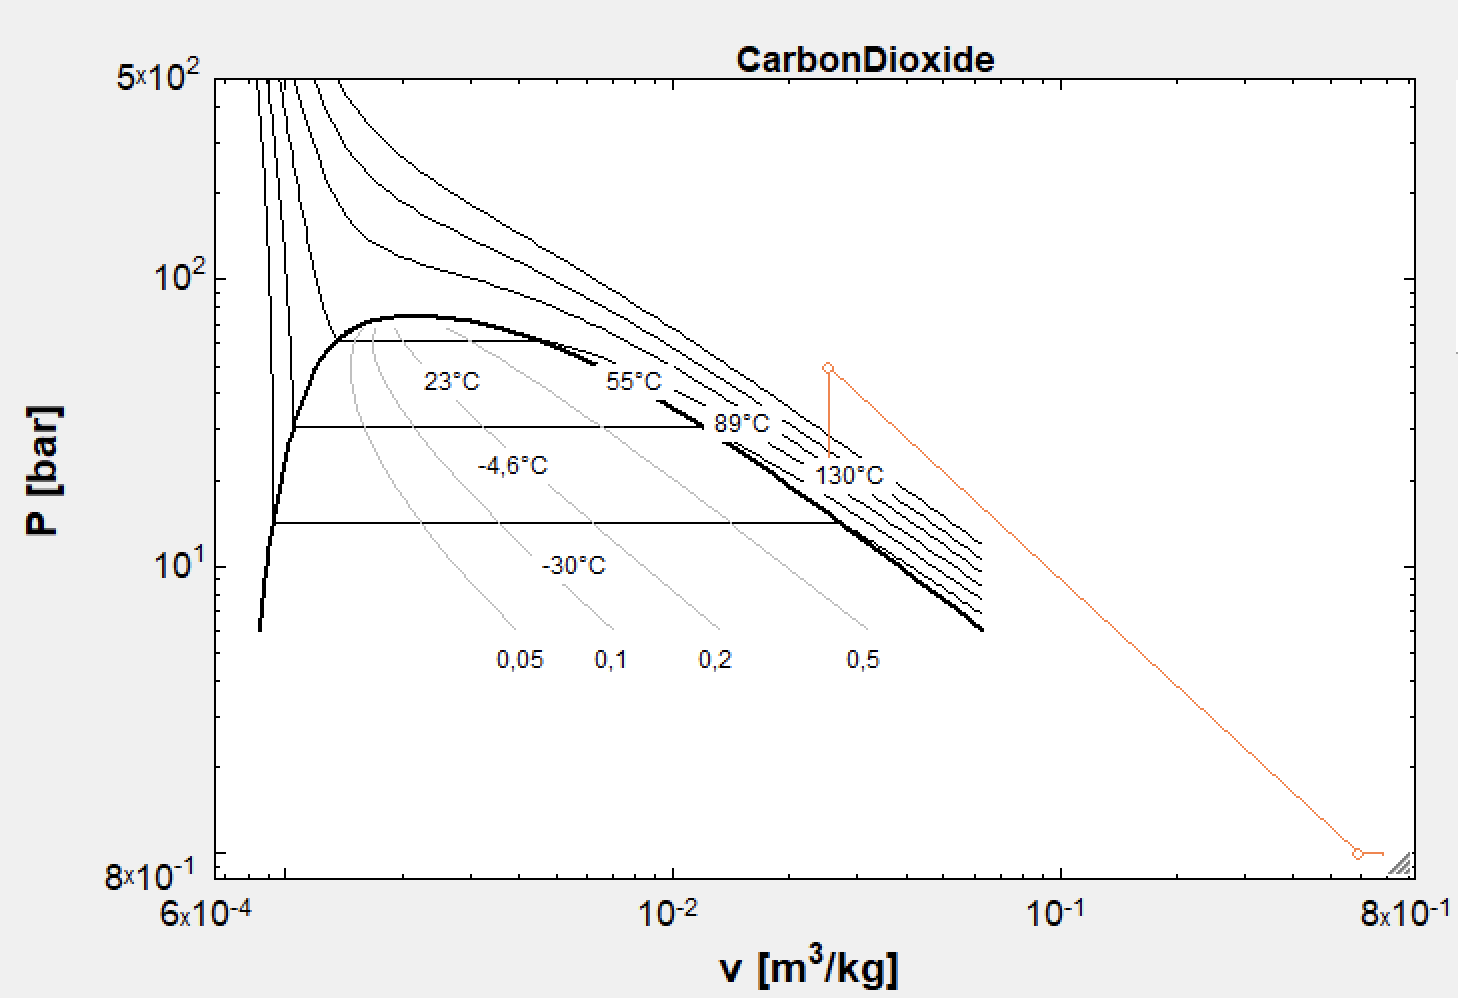
\includegraphics[width=0.5\linewidth]{./figures/p1_4.png}
  \caption{$Pv$-diagram}
  \label{fig:p1_4}
\end{figure}


\opgave{7.}
Tag udgangspunkt i den generelle udgave af termodynamikkens første lov (\textbf{\autoref{eq:t1l}}) og argumenter for at der er enthalpibevarelse for en stationær, adiabatisk strømning gennem en dysse.
\begin{equation}\label{eq:t1l}
  \dot{Q}_{\mathrm{in}} + \dot{W}_{\mathrm{in}} + \sum_{i \in \mathrm{in}} \dot{m}_i \left( h_i + \frac{V_i^2}{2} + gz_i \right) = \dot{Q}_{\mathrm{out}} + \dot{W}_{\mathrm{out}} + \sum_{i \in \mathrm{out}} \dot{m}_i \left( h_i + \frac{V_i^2}{2} + gzi \right) + \frac{\mathrm{d}E}{\mathrm{d}t} 
\end{equation}
For en stationær adiabatisk dysse med ens massestrøm ind og ud af dyssen får vi:
\begin{align*}
  \dot{W}_s &= 0 \\
  \dot{Q} &= 0 \\
  z_1 &\approx z_2 \implies g \Delta z \approx 0 \\
  \dot{m}_1 &= \dot{m}_2 \implies V_1 = V_2
.\end{align*}
Dermed reduceres formlen til:
\[ 
\dot{m} \left( h_1 \right) = \dot{m} \left( h_2 \right) \implies h_1= h_2
.\]
Altså er der entalpibevarelse igennem dyssen.

\opgave{8.}
Tag udgangspunkt i den generelle udgave af termodynamikkens første lov (\textbf{\autoref{eq:t1l}}) og anden lov (\textbf{\autoref{eq:t2l}}) og argumenter for at der altid sker en entropiskabelse i et blandingsbatteri, hvor en varm og kold vandstrøm kommer ind hver for sig og en blanding med homogen temperatur forlader systemet. Antag at der er tale om en stationær strømning.
\begin{equation} \label{eq:t2l}  
  \frac{\dot{Q}_{\mathrm{in}}}{T_{\mathrm{in}}} + \sum_{i \in \mathrm{in}} \dot{m}_i s_i + \dot{S}_{\mathrm{gen}} = \frac{\dot{Q}_{\mathrm{out}}}{T_{\mathrm{out}}} + \sum_{i \in \mathrm{out}} \dot{m}_i s_i + \frac{\mathrm{d}S}{\mathrm{d}t} 
\end{equation}
\bigbreak
For et generelt knudepunkt (som i opgaven) har vi at:
\begin{align*}
  \dot{m}_{\mathrm{cold}} h_{\mathrm{cold}} + \dot{m}_{\mathrm{hot}} h_{\mathrm{hot}} &= \dot{m}_{\mathrm{out}} h_{\mathrm{out}} \\
  \dot{m}_{\mathrm{cold}} + \dot{m}_{\mathrm{hot}} &= \dot{m}_{\mathrm{out}}
.\end{align*}
Entropibalancen giver:
\[ 
\dot{S}_{\mathrm{gen}} = \left( \dot{m}_1 s_1 + \dot{m}_2 s_2 \right)_{\mathrm{in}} - \left( \dot{m}_3 s_3 \right)_{\mathrm{out}} \geq 0
.\]
Der må ske en overførsel af varme $Q$ fra den varme strøm til den kolde. Dermed må entropien for de to strømme ændres som:
\begin{align*}
  \Delta S_{\mathrm{hot}} &= - \frac{Q}{T_{\mathrm{hot}}} \\
  \Delta S_{\mathrm{cold}} &= \frac{Q}{T_{\mathrm{cold}}}
.\end{align*}
Derfor er den totale $\dot{S}_{\mathrm{gen}}$ også:
\[ 
\dot{S}_{\mathrm{gen}} = Q \left( \frac{1}{T_{\mathrm{cold}}} - \frac{1}{T_{\mathrm{hot}}} \right)
.\]
Dermed ses at der altså må genereres en entropi. 

\opgave{9.}
En dampturbine arbejder med et indgangstryk på \qty{10}{bar} og et udgangstryk på \qty{3}{bar}. Indgangstemperaturen er \qty{300}{\celsius}. Turbinen leverer \qty{10}{kW} i stationær drift, og har et varmetab på \qty{1}{kW} til omgivelserne. For at forøge virkningsgraden isoleres turbinen nu, så varmetabet reduceres med 50\%. Det leverede arbejde, trykforholdet og indgangstemperaturen forbliver konstant. Beregn det tabte arbejde før og efter ændringen og vurder hvor meget turbinens virkningsgrad forøges som følge af ændringen.
\bigbreak
Vi kan beregne hele starttilstanden i EES vha. stofdatakald da vi kender to tilstandsstørrelser her. Vi kan dernæst finde tilstand 2s (den isentropiske version af tilstand 2) idet vi her har et nyt tryk og samme entropi som i starttilstanden. Dermed kan det idealiserede specifikke arbejde regnes til:
\[ 
\Delta h = h_2 - h_{2s} = \qty{232}{\frac{kJ}{kg}} 
.\]
En energibalance på dampen giver:
\[ 
\dot{m} \Delta h = W + Q_{\mathrm{tab}} \implies \dot{m} = \frac{W + Q_{\mathrm{tab}}}{\Delta h}
.\]
Før isoleringen er $Q_{tab} = \qty{1}{kW} $ hvilket giver $\dot{m}_{\text{før}} = \qty{0,0474}{\frac{kg}{s}} $ efter isoleringen er $Q_{tab} = \qty{0,50}{kW}$ hvilket giver en ny massestrøm på $\dot{m}_{\text{efter}} = \qty{0,0453}{\frac{kg}{s}}$. Dermed er nyttevirkningen før isoleringen:
\[ 
\eta_{\text{før}} = \frac{10}{11} = 10/11
.\]
Efter isoleringen er den istedet:
\[ 
\eta_{efter} = \frac{10}{\num{10,5}}
.\]


\opgave{10.}
En kølekreds er beskrevet ved følgende skitse \textbf{\autoref{fig:p1_1}}. Kølemidlet er R134a. Lav en EES kode, som beregner følgende i alle nummererede tilstande: Tryk, temperatur, specifik volumen, specifik enthalpi, specifik entropi. Plot derudover et $Ts$-diagram for kredsprocessen.

\begin{figure} [ht]
  \centering
  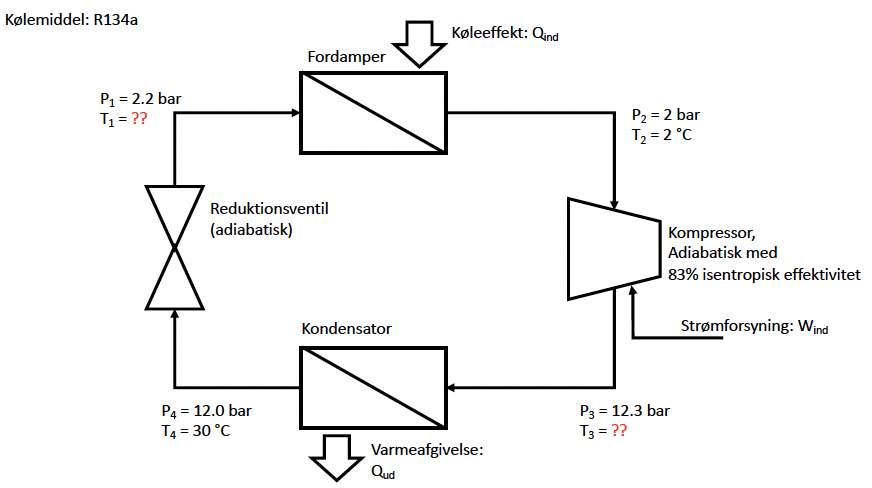
\includegraphics[width=0.5\linewidth]{./figures/p1_1.png}
  \caption{Kølekreds}
  \label{fig:p1_1}
\end{figure}

\opgave{11.}
I brændkammeret på en lille raket motor er trykket \qty{8}{bar}  og temperaturen \qty{1200}{K}. Gassen fra forbrændingen kan antages at opføre sig som en idealgas med $\frac{C_p}{C_v} = \num{1,4} $. Gassen forlader brændkammeret gennem en dysse, hvor den accelereres i en adiabatisk og isentropisk proces. Uden for dyssen er trykket \qty{0,5}{bar} (raketten er allerede i luften). Bestem hastigheden, som gassen forlader dyssen med.

\opgave{12.}
Et elektrolyseapparat laver \qty{21,5}{kg} brint ved brug af \qty{1}{MWh} elektricitet. Beregn førstelovs effektiviteten ift. den øvre brændværdi (HHV) for brint.

\end{document}
